\documentclass[a4paper]{article}
\usepackage[utf8]{inputenc}
\usepackage{amsmath}
\usepackage{graphicx}
\usepackage{mathpazo}
\usepackage{enumitem}
\newlist{myitems}{enumerate}{1}
\setlist[myitems]{label=\arabic*, font=\bfseries, resume}

\begin{document}
\begin{center}

{\huge \textbf{Report on}} \\
\vspace{5mm}
{\huge \textbf{ON THE RATE OF GROWTH OF POPULATION OF THE UNITED STATES SINCE 1790 AND ITS MATHEMATICAL REPRESENTATION}} \\
\vspace{2.5mm}
{\Large \textbf{by Raymond Pearl and Lowell J. Reed  Department of Biometry and Vital Statistic  John Hopkins University}} \\

\vspace{40mm}

To: \\
Professor Timothy Reluga \\

\vspace{10mm}

Report from: \\
Jiaqi Li \\
Yifei Deng\\

\vspace{\fill}

February $28^{th}$, 2018

\clearpage

\textbf{\large{Introduction}} \\

\end{center}

In this paper, we are going to discuss the models made by Raymond Pearl and Lowell J. Reed and how they develop their method in studying population growth. Total of two models are present in details in the paper and we reproduce each of them by three approaches. In particular, the linear least square method is used to reproduced the logarithmic model. Whereas the logistic model is reproduced by explicitly solving the non-linear equations suggested by the author and by non-linear least square method. We also made our own model and compare with the models made by the author. \\

\vspace{10mm}

\begin{center}

\textbf{\large{Background}} \\

\end{center}


In the paper written by Raymond Pearl and Lowell J. Reed, the data of population size for each 10 years from 1790 to 1910 are obtained by census method. In the study of normal rate of population growth, the authors suggested that time interval of 5 years will work better in studying population change. However, population census only takes place once in 10 years. The authors also pointed out the problems of the census estimates that the estimation of the population is made only based on the data given by the last 2 year. This caused the highly inaccuracy of the estimation in a large time interval. Also, the assumptions that "for any given short period of time the population is increasing either in arithmetic or geometric ratio" is inaccurate even for short term. Thus, the author suggests to fit a curve to all the data that is available by using the method of least square. The authors, then, introduced the higher order parabolas. Even though the method of least square should be much better than the census estimates, none of the methods can be absolutely accurate. One problem of the method of least square is the "dangers of extrapolation", as the author mentioned in the paper.\

Other than the "dangers of extrapolation", the author also pointed out some conditions that are not satisfied by the higher order parabolas and the logarithmic parabolas. To solve such a problem, the author introduced a new model that can satisfy the conditions that exist in the real world. As a result, the new model behaves more realistically.\

\vspace{10mm}

\begin{center}

\textbf{\large{Our Work}} \\

\end{center}
 
Before we start to work on the models, we first try to clarify the time interval that is given in the paper so that we could get the value of time (x) as accurate as we can. The author indicates that we should use 1780 as the origin and set 1790 as $x = 1$. Then we calculate the number of days between August $2^{nd}$, 1790 and August $4^{th}$, 1800. This number helps us determine the x value for 1800. Similarly, we will get the x value for all the other years. The chart shown below is the result we get: \

\begin{center}
\begin{tabular}{ |p{1.5cm}||p{2.5cm}|p{2.5cm}| }
 \hline
 \multicolumn{3}{|c|}{Time Interval} \\
 \hline
 Year & Original Date & x in 10 years\\
 \hline
 1790 & August 2nd & 1\\
 1800 & August 4th &  2.00055 \\
 1810 & August 6th & 3.00011\\
 1820 & August 7th & 4.00014\\
 1830 & June 1st & 4.98096\\
 1840 & June 1st & 5.98096 \\
 1850 & June 1st &  6.98096\\
 1860 & June 1st & 7.98096\\
 1870 & June 1st &  8.98096\\
 1880 & June 1st &  9.98096\\
 1890 & June 1st &  10.98096 \\
 1900 & June 1st &  11.98096\\
 1910 & April 15th & 12.96699\\
 \hline
\end{tabular}
\end{center}

Then, we want to take a look at the first model, which is a third order parabola made by Pritchett. In this model, the authors did not discuss much about it. The general form of the model is: \

\begin{center}

$P = A+Bt+Ct^2+Dt^3$\

\end{center}

For this model, the author did not estimate the unknown constants of the model. Instead, he used the data that is already calculated for the third order parabola. Thus, the data we used for the above model is obtained directly from the table that the author made. When we look at this model, we can find that it works fine in the early time intervals, but it overestimates the population size for the last 2 time intervals, just like the author mentioned. (The comparison is made in \textit{Table 1}) \

To make the model better, the author introduced the logarithmic parabola, which was originally designed to estimate the growth of plant. We, then, reproduced this model by the method of linear least square, and the result is as following: \

\begin{center}

$y=9072386-6223289x+841752x^2+19524417 \log{x}$ \

\end{center}

This model shows a much better fit when we compare the error with Pritchett's model as the value of x (time) grows bigger. Thus, our data and results are approximately the same as the author's. The data of the logarithmic model is shown in Table 1 and its plot is shown by figure 1.  \\

However, the author think that this model is not good enough based on the organic laws of population growth. Even though the author admitted that the logarithmic model provides a very high level of accuracy, when time goes to sufficient large value, the population size of the United States would eventually diverge and goes to infinitely large, which in practical it should never happened. Then, the author suggested that the population model should include a point of inflection so that the estimations made by the model would have a boundary.\

\begin{center}
\begin{tabular}{ |p{1cm}|p{1.8cm}|p{1.8cm}|p{1.8cm}|p{1.8cm}|p{1.9cm}| }
 \hline
 \multicolumn{6}{|c|}{Table 1}\\
 \hline
 Year & Observed & Pritchett (a) & Logarithmic (b) & Error of (a) & Error of (b)\\
 \hline
 1790 & 3,929,000 & 4,012,000 & 3,690,849 & 83,000 & -238,151 \\
 1800 & 5,308,000 & 5,267,000 & 5,871,013 & -41,000 & 563,013 \\
 1810 & 7,240,000 & 7,059,000 & 7,293,986 & -181,000 & 53,986 \\
 1820 & 9,638,000 & 9,571,000 & 9,402,506 & -67,000 & -235,494 \\
 1830 & 12,866,000 & 12,985,000 & 12,572,907 & 119,000 & -293,093 \\
 1840 & 17,069,000 & 17,484,000 & 17,128,208 & 415,000 & 59,208 \\
 1850 & 23,192,000 & 23,250,000 & 23,126,599 & 58,000 & -65,402 \\
 1860 & 31,192,000 & 30,465,000 & 30,632,690 & -978,000 & -810,310 \\
 1870 & 38,558,000 & 39,313,000 & 39,688,108 & 755,000 & 1,130,108 \\
 1880 & 50,156,000 & 49,975,000 & 50,321,246 & -181,000 & 165,246 \\
 1890 & 62,948,000 & 62,634,000 & 62,552,341 & -314,000 & -395,659 \\
 1900 & 75,995,000 & 77,472,000 & 76,396,327 & 1,477,000 & 401,327 \\
 1910 & 91,972,000 & 94.673,000 & 91,637,219 & 2,701,000 & -334,781 \\
 \hline
\end{tabular}
\end{center}

\begin{figure}[h]
  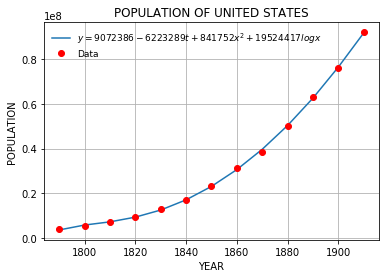
\includegraphics[width=\linewidth]{logarithmic}
  \caption{Logarithmic Parabola}
  \label{fig:1}
\end{figure}


Thus, to obtain an adequate description for the population growth,  the author stated that the following conditions should be satisfied by any model desired:\

\begin{myitems}
\item When time (x) goes to infinity, the population is asymptotic to a boundary $y=k$. \\

Since population size is unable to grow to infinitely large due to organic laws of population growth of a particular community, it is reasonable to say, at some point, that the population growth would have a upper bound.\\

\item When time(x) goes to negative infinity, the population is asymptotic to a boundary $y=0$. \\

No matter how far we trace back for history, the population should always assume to be greater than 0.\\

\item A point of inflection at some point $x = \alpha$ and $y = \beta$. \\

The population would not always increase through time. It may start to decrease after it reaches the highest point due to change of social behavior, development of technology, etc.\\

\item Concave up to the left of $x = \alpha$ and concave down to right of $x = \alpha$. \\

Effects of the point of inflection.\\

\item No horizontal slope except at $x = \pm \infty$. \\

\item Values of $y$ varying continuously from 0 to $k$ as $x$ varies from $-\infty$ to $+\infty$.\\

\end{myitems}

A logistic equation that the author came up that satisfies all requirements above and following the law of population growth is: \

\begin{center}

\hspace{1cm} $y = \dfrac{be^{ax}}{1+ce^{ax}}$      \hspace{0.5cm}      (1)

\end{center}

In this equation, $y$ denotes the population, $x$ denotes time in the scale of 10 years; $a$, $b$ and $c$ are positive constants. \

For simplicities, we took the simplified form of equation (1) for the following steps: \

\begin{center}

$y = \dfrac{b}{e^{-ax}+c}$

\end{center}

According to the author's suggestions, it is sufficient to fit the observations by passing it through three points as the following: \\


\hspace{3.8cm} $(x_1,y_1) = (1, 3929000)$ \

\hspace{3.8cm} $(x_2, y_2) = (6.98096, 23192000)$ \

\hspace{3.8cm} $(x_3, y_3) = (12.96699, 91972000)$ \\


Then, we could reproduce author's work by solving the following non-linear system of equations directly: \

\begin{center}
$3929000 = \dfrac{b}{e^{-a}+c}$ \\ 
$23192000 = \dfrac{b}{e^{-a*6.98096}+c}$ \\ 
$91972000 = \dfrac{b}{e^{-a*12.96699}+c}$ \\
\end{center}

Finally, we will be able to fine the logistic euqation: \

\begin{center}

$y = \dfrac{2927395.3}{e^{- 0.314441x}+ 0.014877}$ \

\end{center}

Then, we can see how this model work by looking at the error between the observed data and the calculated data in Table 2. \

\begin{center}
\begin{tabular}{ |p{1cm}|p{1.8cm}|p{1.8cm}|p{1.8cm}|p{1.9cm}|p{1.9cm}| }
 \hline
 \multicolumn{6}{|c|}{Table 2}\\
 \hline
 Year & Observed & Logistic NLS (a) & Logistic SOE (b)& Error of (a) & Error of (b) \\
 \hline
 1790 & 3,929,000 & 3,939,112 &3,929,000 & 10,112 &0\\
 1800 & 5,308,000 & 5,349,813 &5,342,232 & 41,813 &34,232\\
 1810 & 7,240,000 & 7,244,685 &7,242,525 & 4,685 &2,525\\
 1820 & 9,638,000 & 9,778,004 &9,785,599 & 140,004 &147,598\\
 1830 & 12,866,000 & 13,062,540 &13,085,645 & 196,540 &219,645\\
 1840 & 17,069,000 & 17,443,978 &17,490,926 & 374,978 &421,925\\
 1850 & 23,192,000 & 23,111,304 &23,192,000 & -80,695 &0\\
 1860 & 31,192,000 & 30,310,642 &30,435,847 & -1,132,358 &-1,007,152\\
 1870 & 38,558,000 & 39,249,097 &39,428,326 & 691,097 &870,327\\
 1880 & 50,156,000 & 50,036,565 &50,274,669 & -119,434 &118,669\\
 1890 & 62,948,000 & 62,618,856 &62,911,748 & -329,144 &-36,251\\
 1900 & 75,995,000 & 76,723,627 &77,054,563 & 728,627 &10,595\\
 1910 & 91,972,000 & 91,633,383 &91,972,000 & -338,617 &0\\
 \hline
\end{tabular}
\end{center}

\begin{flushleft}
\footnotesize{*NLS: Method of non-linear least square} \

\footnotesize{*SOE: System of non-linear equations}\\
\end{flushleft}

By comparing the data, we can confirm that our data is approximately the same as the author's.\\

Other than reproducing the author's work by solving the non-linear system directly, we could also implement the method of  non-linear least squares to estimate the unknown constants from the logistic equation. \

During the step of replicating, we used the method of non-linear least squares with an appropriate initial guess: \

\begin{center}

$P_0 = [a=0.03, b=3000, c=0.01]$ \

\end{center}

With the method of non-linear least square, we will find that the logistic equation is: \

\begin{center}

$y = \dfrac{2938284.1}{e^{-0.313233x}+0.014846}$ \\

\end{center}

\vspace{0.4cm}

The plots for the logistic equations solved by fitting data point is shown by figure 2 and by the method of non-linear least squares is shown by figure 3. \

\clearpage

\begin{figure}[h]
  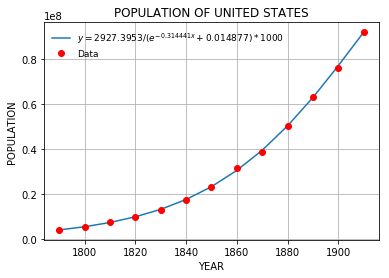
\includegraphics[width=\linewidth]{logistic_fsolve}
  \caption{Logistic Equation Solved by the System of Non-linear Equations}
  \label{fig:2}
  \vspace{2cm}
  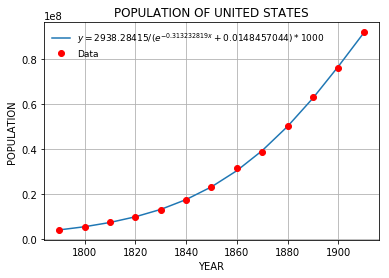
\includegraphics[width=\linewidth]{logistic}
  \caption{Logistic Equation Solved by Method of Non-linear Least Squares}
  \label{fig:3}
\end{figure}

\clearpage

So far, we have successfully reproduced most of the work made by Raymond Pearl and Lowell J. Reed. \

We also want to produce our own models by using what we have learned from class. Thus, by observing the trend of all the data points, we decide to use the exponential law to fit the data. \

First, we make the general form of our model as the following: \

\begin{center}
$y = ke^{rx}$\
\end{center}

Then, we try to estimate the unknown constants, $k$ and $r$, by using the method of least square. As a result, we get the equation for our own model: \

\begin{center}
$y = 3296063.279e^{0.26782946x}$ \
\end{center} 

We also produced the plot for this model: \

\begin{figure}[h]
  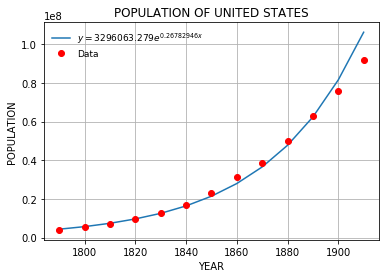
\includegraphics[width=\linewidth]{exponential}
  \caption{Exponential Equation}
  \label{fig:4}
\end{figure}

\vspace{10mm}

As we observe, if we compare our own model with the logistic model, or the logarithmic model, our model overestimates the population at the margin, especially after 1890. This is because the exponential equation is growing much faster than the actual growth rate of population size. \\

\clearpage

\begin{center}
\textbf{\large{Conclusion}} \\
\end{center}

In our work, we went through the process that the author did and successfully reproduced most of the work in the paper. Since the author obtained the logistic equation simply by passing it through three points instead of developing a method to solve for the equation, we tried to find out a method that can solve the equation. By using the method of non-linear least squares, we finally obtain the logistic equation. This model perform well in fitting the data based on the error compared with the logarithmic model. Hence, we think that this model is pretty good and it provides adequate description for the population growth. For the model that we made by ourselves, we find out that a simple model can be very easy to make, but it fits the data poorly. Thus, we can start our work from a simple model, but it is necessary to develop a more complicate model to reach a higher level of accuracy.\

Moreover, by studying this paper, we also find out that a good model can not only make good estimations, but also consider the real world conditions. For the logistic model, it gets the same level of accuracy as the logarithmic model does, and it also satisfies the organic laws of population growth. \

In addition, we think it is worth to mention that there is a typo on page 283 in the paper, where the value a of the equation (xviii) should be 0.313395 instead of what the author stated "0.0313395". \\

\vspace{\fill}

\begin{thebibliography}{9}
\bibitem{knuthwebsite}

Timeanddate.com. Accessed February 28, 2018.  \\
\texttt{https://www.timeanddate.com/}. \\

\end{thebibliography}

\end{document}


